\tikzsetfigurename{module4_2_14_vglCirkel}
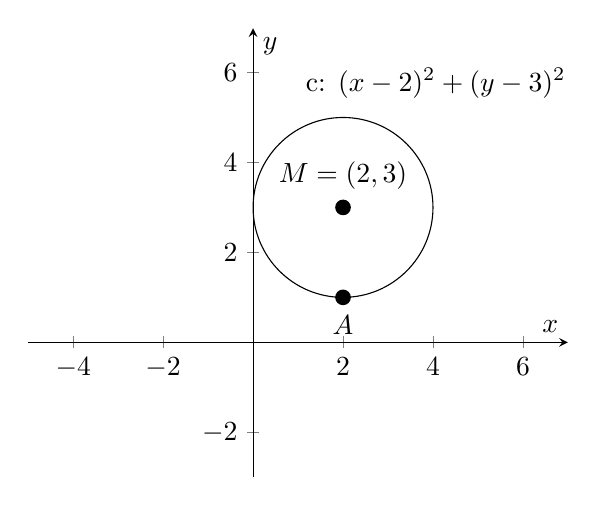
\begin{tikzpicture}
\begin{axis}[xmin=-5, xmax=7, ymin=-1, ymax=5,
axis lines = middle,xlabel=$x$,ylabel=$y$, axis equal]
\draw (axis cs: 2, 3) circle [radius=2];
%	\addplot[red,mark=*] coordinates {(2,3)};
\node[label={90:{$M=(2,3)$}},circle,fill,inner sep=2pt] at (axis cs:2,3) {};
\node[label={270:{$A$}},circle,fill,inner sep=2pt] at (axis cs:2,1) {};
\node[label={90:{c: $(x-2)^2+(y-3)^2=4$}},xshift=1.5cm] at (axis cs:2,5) {};
\end{axis}

%	\begin{axis}[
%	axis lines = left,
%	xmin=-11, xmax=11, ymin=-11, ymax=11,
%	axis equal,
%	xlabel = $x$,
%	ylabel = {$f(x)$},
%	yticklabels={,,}
%	]
%	\draw (axis cs: 0, 0) circle [radius=10];% I've set the radius to 10 only for better show the image
%	\end{axis}

\end{tikzpicture}